\chapter{Linear Programming}
In this chapter we introduce the concept of Linear programming. Most proofs will be omitted but proofs and more in depth explanations can be found in \{some book\}
\section{The structure of a linear program}
In a linear program we want to maximise or minimize a given linear function $z:\R^n \rightarrow \R$ subject to a number of linear inequalities or equalities $g_i:\R^n \rightarrow \R$ with $g_i(x_1,...,x_n)\geq b_i$,$g_i(x_1,...,x_n)\leq b_i$ or $g_i(x_1,...,x_n)= b_i$. The function, $z$, that we want to optimise is called the \textbf{Objective} and the set of inequalities are called the \textbf{Constraints}. A general linear problem is written:
\begin{align}\label{lpform}
\begin{array}{ll@{}ll}
\text{min/max} &z(x_1,...,x_n)&\\
\text{s.t.} &g_1(x_1,...,x_n) \textbf{ ordRel } b_1,&\\
&\vdots&\\
&g_m(x_1,...,x_n) \textbf{ ordRel } b_m&\\
&\text{where each \textbf{ordRel} can be }\leq,\geq \text{ or } =&
\end{array}
\end{align}

\begin{example}\label{lpex}
A maths student wants to save money on his diet while still remaining healthy. To stay healthy his diet must contain at least $b_1=5$ units of protein, $b_2=10$ units of carbs, $b_3=5$ units of fat and $b_4=10$ units of vitamins.\\
He consider buying 3 food products with different nutritional values and prices: \\\\$x_1$ is a take away meal costing 5 and containing 3 units of protein, 12 units of carbs, 7 units of fat and 3 unit of vitamins.\\\\
$x_2$ is a vegetable costing 1 and containing 2 unit of protein, 2 units of carbs, 0 units of fat and 5 units of vitamins.\\\\
$x_3$ is a type of bread costing 2 and containing 1 unit of protein, 4 units of carbs, 2 units of fat and 2 units of vitamins.\\\\
He then define an optimization problem minimizing the cost of food subject to getting the right nutrition
\begin{align}
\begin{array}{ll@{}ll}
\text{min} &5x_1+x_2+2x_3&\\
\text{s.t.} &3x_1+2x_2+x_3 \geq 5,&\\
&12x_1+2x_2+4x_3 \geq 10,&\\
&7x_1+2x_3 \geq 5,&\\
&3x_1+5x_2+2x_3 \geq 10,&\\
\end{array}
\end{align}
\end{example}
\section{feasible and optimal solutions}
\subsection{feasibility}
Given a Linear problem on form \ref{lpform} any point of $\R^n$ such that all $m$ constraints are true is called a feasible solution. The set of all these points is called the feasible set. In the case \Cref{lpex} the feasible set is the set of all combinations of amounts of the different foods such that the nutritional requirements are met. If a problem has no feasible solutions, that problem is said to be infeasible. A feasibility problem is a special case in linear programming where our object function is constant and thus if any feasible solution exists, that solution is optimal.
\subsection{optimal solutions}
A feasible solution $\textbf{x}_0 \in \R^n$ is said to be optimal if $z(\textbf{x}_0) \geq z(\textbf{x}_0)$ (when maximizing) or $z(\textbf{x}_0) \leq z(\textbf{x}_0)$ (when minimizing) for all feasible solutions $\textbf{x} \in \R^n$.\\\\
- something about unbounded feasible sets.\\\\
- something about the result where an optimal solution is always in an extreme point of the polyhedron, leading us into the convexity and simplex part.
\section{Convexity}
\begin{definition}\label{convex}
A set $X \in \R^n$ is said to be convex if for any two points $a, b \in X$ the straight line segment 
%$\{x|x=(1-t)a+tb,t\in [0,1]\}$
connecting $a$ and $b$ is entirely within $X$.
\end{definition}
\begin{theorem}
A feasible region of a linear program is convex
\begin{proof}
easy short proof
\end{proof}
\end{theorem}
\section{The geometric/graphical intuition}
Section with pretty 3d polyhedron and a objective plane of \Cref{lpex} once i figure out how to use TikZ. \todo{learn TikZ} 
\section{Matrix representation of an LP and Slack variables}
Since the objective function and the constraints of a linear program are all linear functions we can also write a linear program using matrix-vector products. \\
The object can be written as the product of the vector of variables to be determined 
$\begin{bmatrix}x_{1} \\           x_{2} \\
\vdots \\
x_{n}
\end{bmatrix}=\textbf{x}$, and the transposed vector of coefficients $[c_1,c_2,...,c_n]=\textbf{c}^T$ of each $x_i$ in the objective.\\
Likewise the constraints can be written as the matrix-vector products of $n\times m$ constraint matrices,$A$ where $m$ is the number of a constraints with a certain order relation, and $\textbf{x}$ with some order relation ($\leq,\geq or =)$ to a $1\times m$ vector $\textbf{b}$.\\
Rewriting any $\leq$ constraint to $\geq$ in case of minimization or any $\geq$ to $\leq$ in case of maximization (the equality constraints can be written with two inequalities) we can write the linear program on it's \textit{canonical form}:
\begin{align}\label{canonicalMin}
\begin{array}{ll@{}ll}
\text{min} &\textbf{c}^T\textbf{x}&\\
\text{s.t.} &A\textbf{x} \geq \textbf{b},&\\
&\textbf{x} \geq 0,&\\
\end{array}
\end{align}
\begin{align}\label{canonicalMax}
\begin{array}{ll@{}ll}
\text{max} &\textbf{c}^T\textbf{x}&\\
\text{s.t.} &A\textbf{x} \leq \textbf{b},&\\
&\textbf{x} \geq 0,&\\
\end{array}
\end{align}
in case of \Cref{lpex} we write it on it's canonical form:
\begin{align}
\begin{array}{ll@{}ll}
\text{min} &[5,1,2]\begin{bmatrix}x_{1} \\x_{2} \\x_{3}\end{bmatrix}&\\
\text{s.t.} &\begin{bmatrix}3&2&1 \\12&2&4 \\7&0&2\\3&5&2\end{bmatrix}\begin{bmatrix}x_{1} \\x_{2} \\x_{3}\end{bmatrix} \geq \begin{bmatrix}5 \\10 \\5\\10\end{bmatrix},&\\
&\textbf{x} \geq 0,&\\
\end{array}
\end{align}
Much like how we made an LP on canonical form by manipulating the inequalities, we can also write any LP on it's \textit{standard form} 
\begin{align}
\begin{array}{ll@{}ll}
\text{max/min} &\textbf{c}^T\textbf{x}&\\
\text{s.t.} &A\textbf{x} = \textbf{b},&\\
&\textbf{x} \geq 0,&\\
\end{array}
\end{align}
by introducing a $1\times m$ vector, $\textbf{s}$, with one slack variable for each constraint and thus creating a new LP on standard with the same solutions as the old one.
\begin{align}
\begin{array}{ll@{}ll}
\text{max} &\textbf{c}^T\textbf{x}&\\
\text{s.t.} &A\textbf{x}+\textbf{s} =\textbf{b},&\\
&\textbf{x,s} \geq 0,&\\
\end{array}
\end{align}
These forms and the concept of slack variables will come in handy later (I hope)
\section{Duality}
Another important result in Linear programming is the concept of duality.
\begin{definition}
Given a maximization linear program on canonical form \ref{canonicalMax}
We define it's dual problem as the minimization problem:
\begin{align}\label{canonicalMaxDual}
\begin{array}{ll@{}ll}
\text{min} &\textbf{b}^T\textbf{y}&\\
\text{s.t.} &A^T\textbf{y} \geq \textbf{c},&\\
&\textbf{y} \geq 0,&\\
\end{array}
\end{align}
\end{definition}
\begin{theorem}
An optimal solution to a linear program on it's primal form is also optimal in the dual form
\begin{proof}
proof
\end{proof}
\end{theorem}
\subsection{Weak and strong duality}
\section{Worst case runtime of an LP}
This might be relevant since linear programming is in P and integer programming is NP-hard.
\section{The simplex method}
Result showing that Linear programming is in P.

\iffalse
\section{bibtex}
I den øverste mappe er der en mappe der hedder preamble. Hvis man åbne preamble.tex, vil man se noget kode alá
\begin{center}
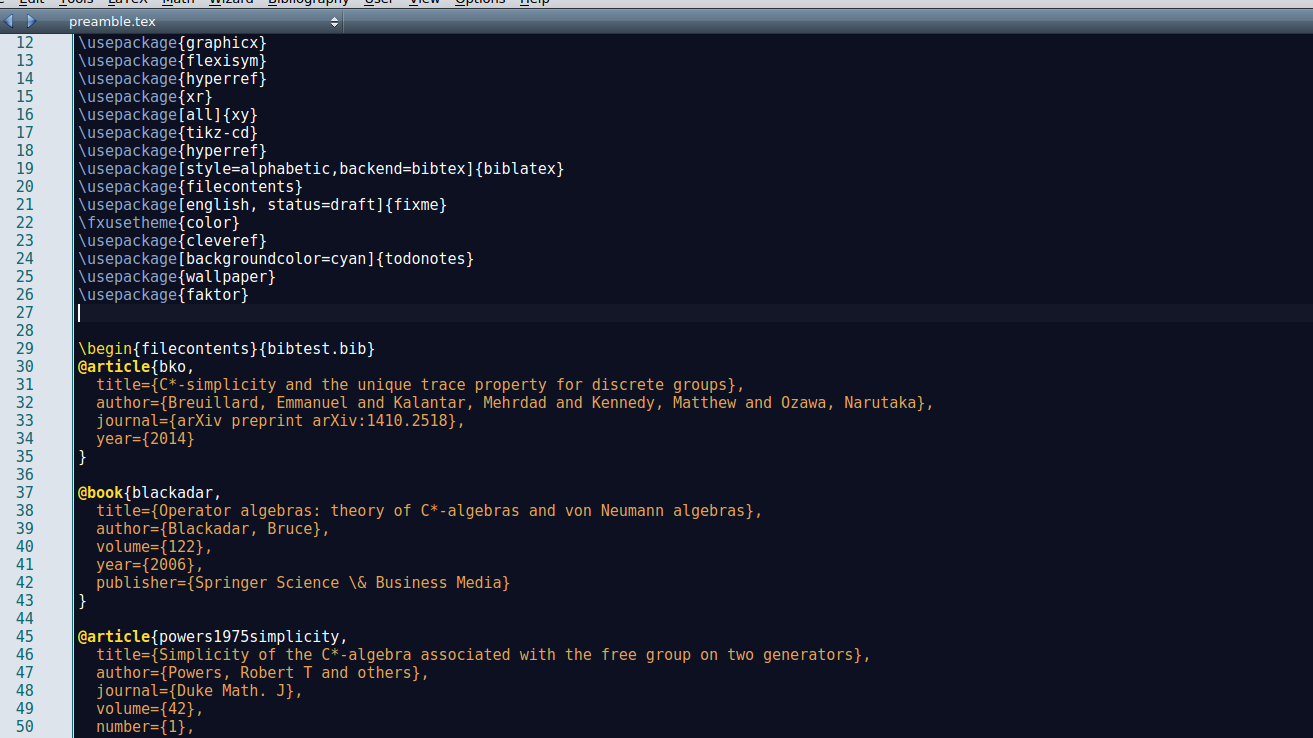
\includegraphics[scale=0.2]{figure/1.png}\\
\end{center}
De dele af koden som starter med fx @book laver en reference til bogen alá \begin{center}
\cite[Proposition 5][7]{zhu}
\end{center} Man behøver ikke skrive dette selv manuelt, man kan nemlig gå ind på \href{https://scholar.google.dk/}{Google scholar} og søge på en bog, og så dukker der en valgmulighed op til at kopiere bibtex kode. Se figuren nedenunder!

\begin{center}
\framebox{
\includegraphics[scale=0.4]{figure/2.png}}\\
\framebox{\texttt{step 1.}}\\
\framebox{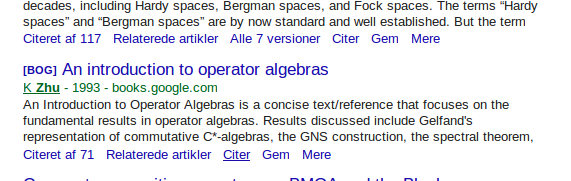
\includegraphics[scale=0.4]{figure/3.png}}\\
\framebox{\texttt{step 2.}}\\
\framebox{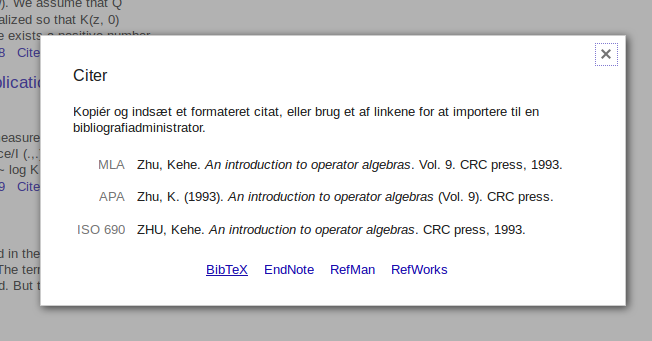
\includegraphics[scale=0.4]{figure/4.png}}\\
\framebox{\texttt{step 3.}}\\
\framebox{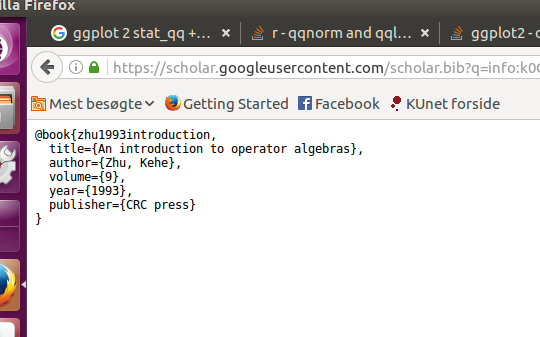
\includegraphics[scale=0.4]{figure/5.png}}\\
\framebox{\texttt{step 4.}}
\end{center}

\begin{remark}
Notér venligst, at for at få latex til at compile ens bibtex, skal man sætte Latex til at compile det manuelt. I Texmaker gøres det på følgende måde: Klik options -> configure texmaker -> build options og vælg PDFlatex + Biblatex + 2x pdflatex +view pdf, som set på nedestående billede:
\begin{center}
\framebox{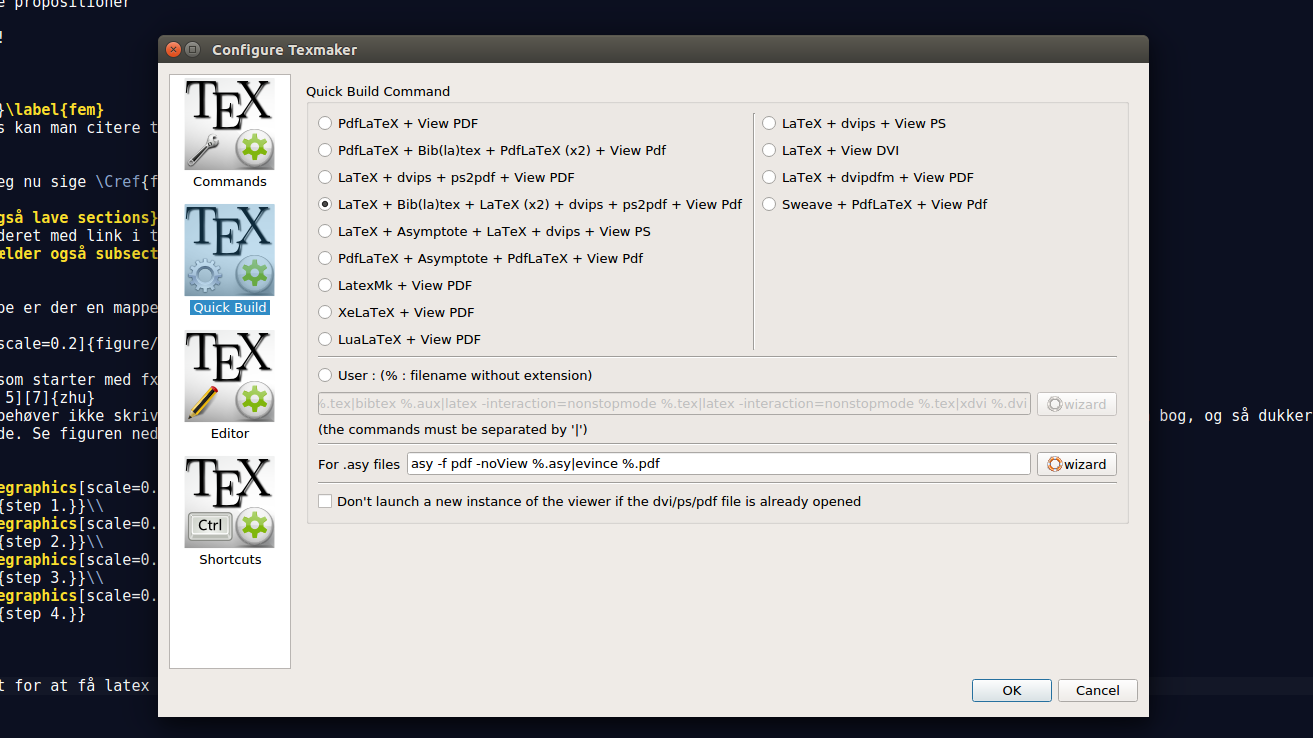
\includegraphics[scale=0.3]{figure/6.png}}
\end{center}
Og lige som det sidste: hvis man ikke citérer en text man har inkluderet, så dukker den ikke op på ens "bibliography". Så hvis man har 9 bøger i ens kode, men har citeret 0, så dukker intet "biblography" chapter op i dokumentet!
\end{remark}
\fi